\documentclass{article}\usepackage[]{graphicx}\usepackage[]{xcolor}
% maxwidth is the original width if it is less than linewidth
% otherwise use linewidth (to make sure the graphics do not exceed the margin)
\makeatletter
\def\maxwidth{ %
  \ifdim\Gin@nat@width>\linewidth
    \linewidth
  \else
    \Gin@nat@width
  \fi
}
\makeatother

\definecolor{fgcolor}{rgb}{0.345, 0.345, 0.345}
\newcommand{\hlnum}[1]{\textcolor[rgb]{0.686,0.059,0.569}{#1}}%
\newcommand{\hlsng}[1]{\textcolor[rgb]{0.192,0.494,0.8}{#1}}%
\newcommand{\hlcom}[1]{\textcolor[rgb]{0.678,0.584,0.686}{\textit{#1}}}%
\newcommand{\hlopt}[1]{\textcolor[rgb]{0,0,0}{#1}}%
\newcommand{\hldef}[1]{\textcolor[rgb]{0.345,0.345,0.345}{#1}}%
\newcommand{\hlkwa}[1]{\textcolor[rgb]{0.161,0.373,0.58}{\textbf{#1}}}%
\newcommand{\hlkwb}[1]{\textcolor[rgb]{0.69,0.353,0.396}{#1}}%
\newcommand{\hlkwc}[1]{\textcolor[rgb]{0.333,0.667,0.333}{#1}}%
\newcommand{\hlkwd}[1]{\textcolor[rgb]{0.737,0.353,0.396}{\textbf{#1}}}%
\let\hlipl\hlkwb

\usepackage{framed}
\makeatletter
\newenvironment{kframe}{%
 \def\at@end@of@kframe{}%
 \ifinner\ifhmode%
  \def\at@end@of@kframe{\end{minipage}}%
  \begin{minipage}{\columnwidth}%
 \fi\fi%
 \def\FrameCommand##1{\hskip\@totalleftmargin \hskip-\fboxsep
 \colorbox{shadecolor}{##1}\hskip-\fboxsep
     % There is no \\@totalrightmargin, so:
     \hskip-\linewidth \hskip-\@totalleftmargin \hskip\columnwidth}%
 \MakeFramed {\advance\hsize-\width
   \@totalleftmargin\z@ \linewidth\hsize
   \@setminipage}}%
 {\par\unskip\endMakeFramed%
 \at@end@of@kframe}
\makeatother

\definecolor{shadecolor}{rgb}{.97, .97, .97}
\definecolor{messagecolor}{rgb}{0, 0, 0}
\definecolor{warningcolor}{rgb}{1, 0, 1}
\definecolor{errorcolor}{rgb}{1, 0, 0}
\newenvironment{knitrout}{}{} % an empty environment to be redefined in TeX

\usepackage{alltt}
\usepackage[margin=1.0in]{geometry} % To set margins
\usepackage{amsmath}  % This allows me to use the align functionality.
                      % If you find yourself trying to replicate
                      % something you found online, ensure you're
                      % loading the necessary packages!
\usepackage{amsfonts} % Math font
\usepackage{fancyvrb}
\usepackage{hyperref} % For including hyperlinks
\usepackage[shortlabels]{enumitem}% For enumerated lists with labels specified
                                  % We had to run tlmgr_install("enumitem") in R
\usepackage{float}    % For telling R where to put a table/figure
\usepackage{natbib}        %For the bibliography
\bibliographystyle{apalike}%For the bibliography
\IfFileExists{upquote.sty}{\usepackage{upquote}}{}
\begin{document}


\cite{Kasdin25} show that dopamine in the brains of young zebra finches acts as 
a learning signal, increasing when they sing closer to their adult song and 
decreasing when they sing further away, effectively guiding their vocal 
development through trial-and-error. This suggests that complex natural 
behaviors, like learning to sing, are shaped by dopamine-driven reinforcement 
learning, similar to how artificial intelligence learns. You can find the 
paper at this link:
\href{https://www.nature.com/articles/s41586-025-08729-1}{{https://www.nature.com/articles/s41586-025-08729-1}.}.

Note they measure dopamine using fibre photometry, changes in the fluorescence
indicate dopamine changes in realtime. Their specific measurement considers 
changes in flourescence in 100-ms windows between 200 and 300 ms from the start 
of singing, averaged across development.

\begin{enumerate}
%%%%%%%%%%%%%%%%%%%%%%%%%%%%%%%%%%%%%%%%%%%%%%%%%%%%%%%%%%%%%%%%%
% CONDUCT A POWER ANALYSIS
%%%%%%%%%%%%%%%%%%%%%%%%%%%%%%%%%%%%%%%%%%%%%%%%%%%%%%%%%%%%%%%%%
\item Using the \texttt{pwr} package for \texttt{R} \citep{pwr},
conduct a power analysis. How many observations would the researchers 
need to detect a moderate-to-large effect ($d=0.65$) when using 
$\alpha=0.05$ and default power (0.80) for a two-sided one sample 
$t$ test.
\begin{knitrout}
\definecolor{shadecolor}{rgb}{0.969, 0.969, 0.969}\color{fgcolor}\begin{kframe}
\begin{alltt}
\hlkwd{library}\hldef{(pwr)}
\hldef{(}\hlkwd{pwr.t.test}\hldef{(}\hlkwc{d} \hldef{=} \hlnum{0.65}\hldef{,} \hlcom{# large effect}
           \hlkwc{power} \hldef{=} \hlnum{0.80}\hldef{,}
           \hlkwc{sig.level} \hldef{=} \hlnum{0.05}\hldef{,}
           \hlkwc{alternative} \hldef{=} \hlsng{"two.sided"}\hldef{,}
           \hlkwc{type} \hldef{=} \hlsng{"one.sample"}\hldef{))}
\end{alltt}
\begin{verbatim}
## 
##      One-sample t test power calculation 
## 
##               n = 20.58039
##               d = 0.65
##       sig.level = 0.05
##           power = 0.8
##     alternative = two.sided
\end{verbatim}
\end{kframe}
\end{knitrout}
When we perform two-sample one-sided t-test with with power = 0.80,
and $\alpha$ = 0.05, we get an output of n = 20.58039. 
So, to detect a moderate-to-large effect (d= 0.65), the researchers
must use atleast 21 observations.
%%%%%%%%%%%%%%%%%%%%%%%%%%%%%%%%%%%%%%%%%%%%%%%%%%%%%%%%%%%%%%%%%
% COLLECT DATA
%%%%%%%%%%%%%%%%%%%%%%%%%%%%%%%%%%%%%%%%%%%%%%%%%%%%%%%%%%%%%%%%%
\item Click the link to go to the paper. Find the source data for 
Figure 2. Download the Excel file. Describe what you needed to
do to collect the data for Figure 2(g). Note that you only need the 
\texttt{closer\_vals} and \texttt{further\_vals}. Ensure to 
\texttt{mutate()} the data to get a difference 
(e.g., \texttt{closer\_vals - further\_vals}).

To collect the data for Figure2(g), we had to download the Excel file from the link 
and then isolate the two specific Excel sheets we wanted; which 
were the closer values sheet and the farther values sheet. 
Then, we combined the two Excel sheets and saved them to a csv
which we then read with \verb|read_csv|.
Finally, we used mutate to create a difference column which was calculated
by subtracting the closer value column from the farther value column.
%%%%%%%%%%%%%%%%%%%%%%%%%%%%%%%%%%%%%%%%%%%%%%%%%%%%%%%%%%%%%%%%%
% SUMMARIZE DATA
%%%%%%%%%%%%%%%%%%%%%%%%%%%%%%%%%%%%%%%%%%%%%%%%%%%%%%%%%%%%%%%%%
\newpage
\item Summarize the data.
\begin{enumerate}
  \item Summarize the further data. Do the data suggest that
   dopamine in the brains of young zebra finches decreases when
   they sing further away?
\begin{knitrout}
\definecolor{shadecolor}{rgb}{0.969, 0.969, 0.969}\color{fgcolor}

{\centering 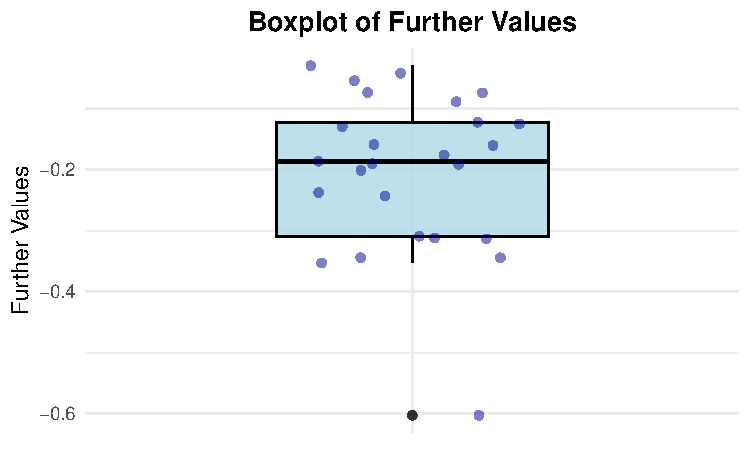
\includegraphics[width=\maxwidth]{figure/unnamed-chunk-3-1} 

}


\end{knitrout}
% latex table generated in R 4.4.2 by xtable 1.8-4 package
% Thu Apr 17 12:29:23 2025
\begin{table}[ht]
\centering
\begin{tabular}{rrrrrr}
  \hline
mean\_further & sd\_further & median\_further & IQR\_further & skewness\_further & exkurtosis\_further \\ 
  \hline
-0.203 & 0.130 & -0.187 & 0.187 & -1.036 & 1.192 \\ 
   \hline
\end{tabular}
\end{table}

The data suggest that dopamine in the brains of young zebra finches decreases when they sing further away
since the mean and median are both negative. Looking at the boxplot, it is abundantly clear
that nearly all of the points are negative, further showing that the dopamine in the brans of young zebra
fiches decreases when they sing further away.


   \item Summarize the closer data. Do the data suggest that
   dopamine in the brains of young zebra finches increases when
   they sing closer to their adult song?
\begin{knitrout}
\definecolor{shadecolor}{rgb}{0.969, 0.969, 0.969}\color{fgcolor}

{\centering 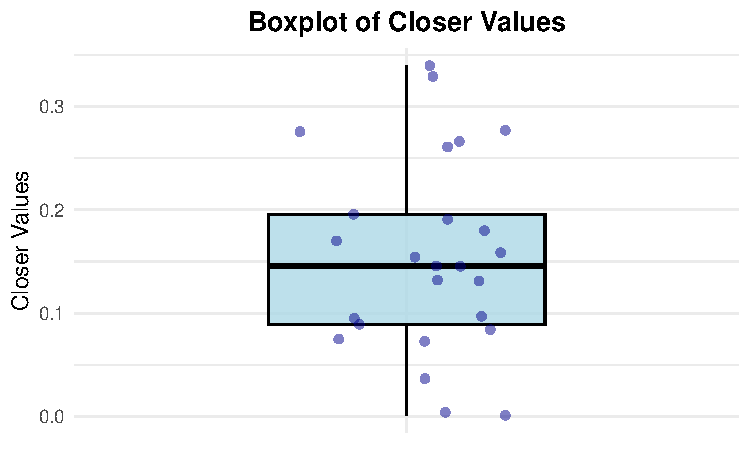
\includegraphics[width=\maxwidth]{figure/unnamed-chunk-5-1} 

}


\end{knitrout}
% latex table generated in R 4.4.2 by xtable 1.8-4 package
% Thu Apr 17 12:29:23 2025
\begin{table}[ht]
\centering
\begin{tabular}{rrrrrr}
  \hline
mean\_closer & sd\_closer & median\_closer & IQR\_closer & skewness\_closer & exkurtosis\_closer \\ 
  \hline
0.156 & 0.094 & 0.146 & 0.107 & 0.295 & -0.859 \\ 
   \hline
\end{tabular}
\end{table}

The data suggest that dopamine in the brains of young zebra finches increases when they sing further away
since the mean and median are both positive Looking at the boxplot, it is abundantly clear
that nearly all of the points are positive, further showing that the dopamine in the brans of young zebra
fiches increases when they sing further away.


  \item Summarize the paired differences. Do the data suggest
  that there is a difference between dopamine in the brains of
  young zebra finches when they sing further away compared to 
  closer to their adult song?
\begin{knitrout}
\definecolor{shadecolor}{rgb}{0.969, 0.969, 0.969}\color{fgcolor}

{\centering 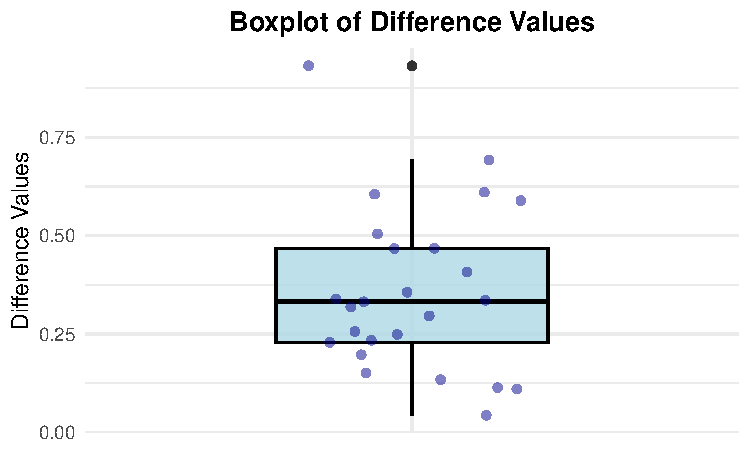
\includegraphics[width=\maxwidth]{figure/unnamed-chunk-7-1} 

}


\end{knitrout}
% latex table generated in R 4.4.2 by xtable 1.8-4 package
% Thu Apr 17 12:29:23 2025
\begin{table}[ht]
\centering
\begin{tabular}{rrrrrr}
  \hline
mean\_difference & sd\_difference & median\_difference & IQR\_difference & skewness\_difference & exkurtosis\_difference \\ 
  \hline
0.359 & 0.211 & 0.332 & 0.239 & 0.773 & 0.128 \\ 
   \hline
\end{tabular}
\end{table}

The data suggest that there is a difference between dopamine in the brains of young zebra finches when they sing further away from their adultsong compared to closer to their adultsong. If there were no difference, we would expect all of the data points to be around zero and for the mean and median to both be around zero. However, all of these values are positive, indicating that dopamine levels are generally higher when the birds sing closer to their adultsong. Therefore, we have reason to believe that there may be a difference between dopamine in the brains of young zebra finches when they sing further away compared to closer to their adultsong.
\end{enumerate}
%%%%%%%%%%%%%%%%%%%%%%%%%%%%%%%%%%%%%%%%%%%%%%%%%%%%%%%%%%%%%%%%%
% CONDUCT THE TESTS
%%%%%%%%%%%%%%%%%%%%%%%%%%%%%%%%%%%%%%%%%%%%%%%%%%%%%%%%%%%%%%%%%
\item Conduct the inferences they do in the paper. Make sure to report the results
a little more comprehensively -- that is your parenthetical should look something
like: ($t=23.99$, $p<0.0001$; $g=1.34$; 95\% CI: 4.43, 4.60).\\
\textbf{Note:} Your numbers may vary slightly as they performed some unclear
correction of their $p$-values. I'm waiting to hear back from them via email!
\begin{enumerate}
  \item ``The close responses differed significantly from 0 ($p=1.63 \times 10^{-8}$).''
\newline ($t=8.3024$, $p<0.0001$; $g=1.61$; 95\% CI: 0.1173875, 0.1950586).
  \item ``The far responses differed significantly from 0 ($p=5.17 \times 10^{-8}$).''
\newline ($t=-7.778$, $p<0.0001$; $g=-1.51$; 95\% CI: -0.2565176, -0.1489313).
  \item ``The difference between populations was significant ($p=1.04 \times10^{-8}$).''
\newline ($t=8.5109$, $p<0.0001$; $g=1.65$; 95\% CI: 0.2719028, 0.4459921).
\end{enumerate}
%%%%%%%%%%%%%%%%%%%%%%%%%%%%%%%%%%%%%%%%%%%%%%%%%%%%%%%%%%%%%%%%%
% CONDUCT THE TESTS
%%%%%%%%%%%%%%%%%%%%%%%%%%%%%%%%%%%%%%%%%%%%%%%%%%%%%%%%%%%%%%%%%
\newpage
\item Reverse engineer the hypothesis test plot from Lecture 20 to create accurate
hypothesis testing plots for each part of the previous question.
\begin{enumerate}
  \item Question 4, part(a).
\begin{knitrout}
\definecolor{shadecolor}{rgb}{0.969, 0.969, 0.969}\color{fgcolor}

{\centering 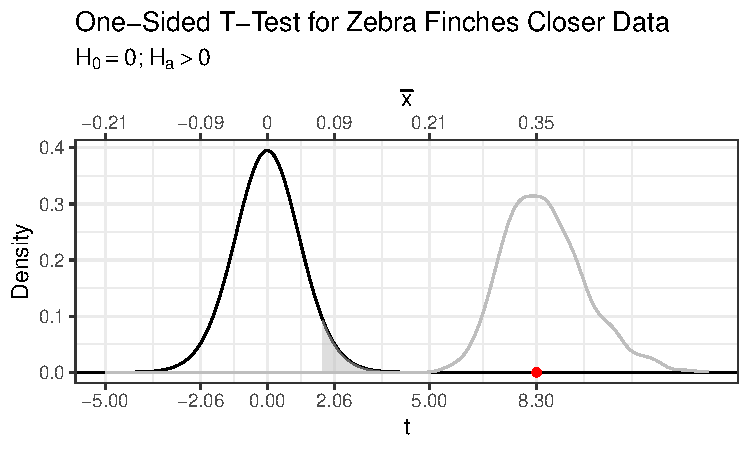
\includegraphics[width=\maxwidth]{figure/unnamed-chunk-9-1} 

}


\end{knitrout}
  \item Question 4, part(b).
\begin{knitrout}
\definecolor{shadecolor}{rgb}{0.969, 0.969, 0.969}\color{fgcolor}

{\centering 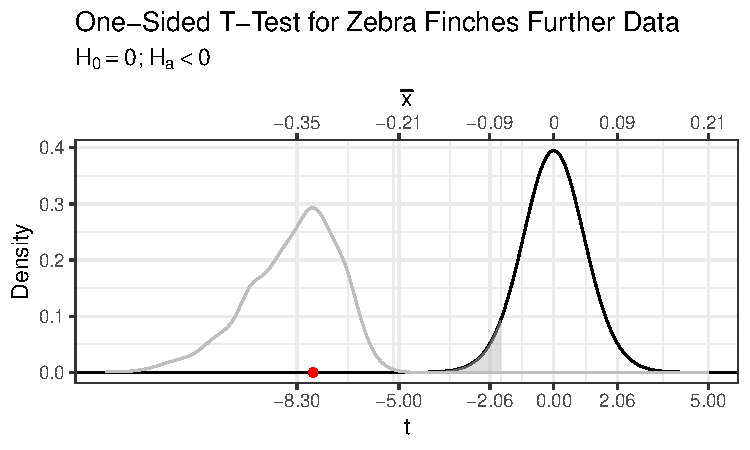
\includegraphics[width=\maxwidth]{figure/unnamed-chunk-10-1} 

}


\end{knitrout}
\newpage
  \item Question 4, part(c).
\begin{knitrout}
\definecolor{shadecolor}{rgb}{0.969, 0.969, 0.969}\color{fgcolor}

{\centering 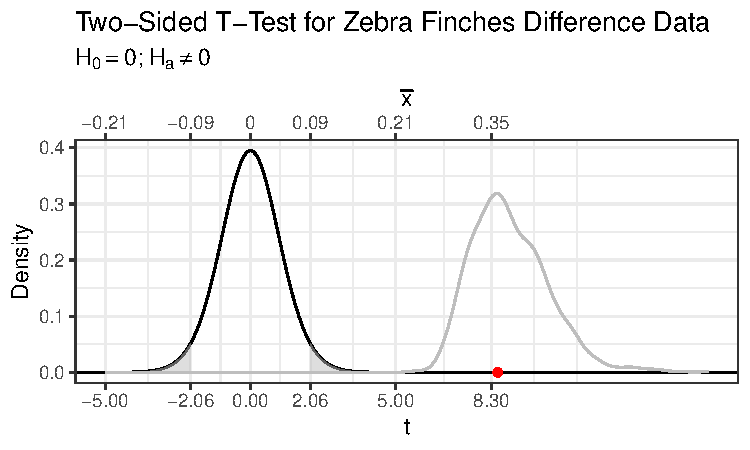
\includegraphics[width=\maxwidth]{figure/unnamed-chunk-11-1} 

}


\end{knitrout}
\end{enumerate}
\end{enumerate}


\bibliography{bibliography}
\end{document}
